\documentclass[1p]{elsarticle_modified}
%\bibliographystyle{elsarticle-num}

%\usepackage[colorlinks]{hyperref}
%\usepackage{abbrmath_seonhwa} %\Abb, \Ascr, \Acal ,\Abf, \Afrak
\usepackage{amsfonts}
\usepackage{amssymb}
\usepackage{amsmath}
\usepackage{amsthm}
\usepackage{scalefnt}
\usepackage{amsbsy}
\usepackage{kotex}
\usepackage{caption}
\usepackage{subfig}
\usepackage{color}
\usepackage{graphicx}
\usepackage{xcolor} %% white, black, red, green, blue, cyan, magenta, yellow
\usepackage{float}
\usepackage{setspace}
\usepackage{hyperref}

\usepackage{tikz}
\usetikzlibrary{arrows}

\usepackage{multirow}
\usepackage{array} % fixed length table
\usepackage{hhline}

%%%%%%%%%%%%%%%%%%%%%
\makeatletter
\renewcommand*\env@matrix[1][\arraystretch]{%
	\edef\arraystretch{#1}%
	\hskip -\arraycolsep
	\let\@ifnextchar\new@ifnextchar
	\array{*\c@MaxMatrixCols c}}
\makeatother %https://tex.stackexchange.com/questions/14071/how-can-i-increase-the-line-spacing-in-a-matrix
%%%%%%%%%%%%%%%

\usepackage[normalem]{ulem}

\newcommand{\msout}[1]{\ifmmode\text{\sout{\ensuremath{#1}}}\else\sout{#1}\fi}
%SOURCE: \msout is \stkout macro in https://tex.stackexchange.com/questions/20609/strikeout-in-math-mode

\newcommand{\cancel}[1]{
	\ifmmode
	{\color{red}\msout{#1}}
	\else
	{\color{red}\sout{#1}}
	\fi
}

\newcommand{\add}[1]{
	{\color{blue}\uwave{#1}}
}

\newcommand{\replace}[2]{
	\ifmmode
	{\color{red}\msout{#1}}{\color{blue}\uwave{#2}}
	\else
	{\color{red}\sout{#1}}{\color{blue}\uwave{#2}}
	\fi
}

\newcommand{\Sol}{\mathcal{S}} %segment
\newcommand{\D}{D} %diagram
\newcommand{\A}{\mathcal{A}} %arc


%%%%%%%%%%%%%%%%%%%%%%%%%%%%%5 test

\def\sl{\operatorname{\textup{SL}}(2,\Cbb)}
\def\psl{\operatorname{\textup{PSL}}(2,\Cbb)}
\def\quan{\mkern 1mu \triangleright \mkern 1mu}

\theoremstyle{definition}
\newtheorem{thm}{Theorem}[section]
\newtheorem{prop}[thm]{Proposition}
\newtheorem{lem}[thm]{Lemma}
\newtheorem{ques}[thm]{Question}
\newtheorem{cor}[thm]{Corollary}
\newtheorem{defn}[thm]{Definition}
\newtheorem{exam}[thm]{Example}
\newtheorem{rmk}[thm]{Remark}
\newtheorem{alg}[thm]{Algorithm}

\newcommand{\I}{\sqrt{-1}}
\begin{document}

%\begin{frontmatter}
%
%\title{Boundary parabolic representations of knots up to 8 crossings}
%
%%% Group authors per affiliation:
%\author{Yunhi Cho} 
%\address{Department of Mathematics, University of Seoul, Seoul, Korea}
%\ead{yhcho@uos.ac.kr}
%
%
%\author{Seonhwa Kim} %\fnref{s_kim}}
%\address{Center for Geometry and Physics, Institute for Basic Science, Pohang, 37673, Korea}
%\ead{ryeona17@ibs.re.kr}
%
%\author{Hyuk Kim}
%\address{Department of Mathematical Sciences, Seoul National University, Seoul 08826, Korea}
%\ead{hyukkim@snu.ac.kr}
%
%\author{Seokbeom Yoon}
%\address{Department of Mathematical Sciences, Seoul National University, Seoul, 08826,  Korea}
%\ead{sbyoon15@snu.ac.kr}
%
%\begin{abstract}
%We find all boundary parabolic representation of knots up to 8 crossings.
%
%\end{abstract}
%\begin{keyword}
%    \MSC[2010] 57M25 
%\end{keyword}
%
%\end{frontmatter}

%\linenumbers
%\tableofcontents
%
\newcommand\colored[1]{\textcolor{white}{\rule[-0.35ex]{0.8em}{1.4ex}}\kern-0.8em\color{red} #1}%
%\newcommand\colored[1]{\textcolor{white}{ #1}\kern-2.17ex	\textcolor{white}{ #1}\kern-1.81ex	\textcolor{white}{ #1}\kern-2.15ex\color{red}#1	}

{\Large $\underline{12n_{0246}~(K12n_{0246})}$}

\setlength{\tabcolsep}{10pt}
\renewcommand{\arraystretch}{1.6}
\vspace{1cm}\begin{tabular}{m{100pt}>{\centering\arraybackslash}m{274pt}}
\multirow{5}{120pt}{
	\centering
	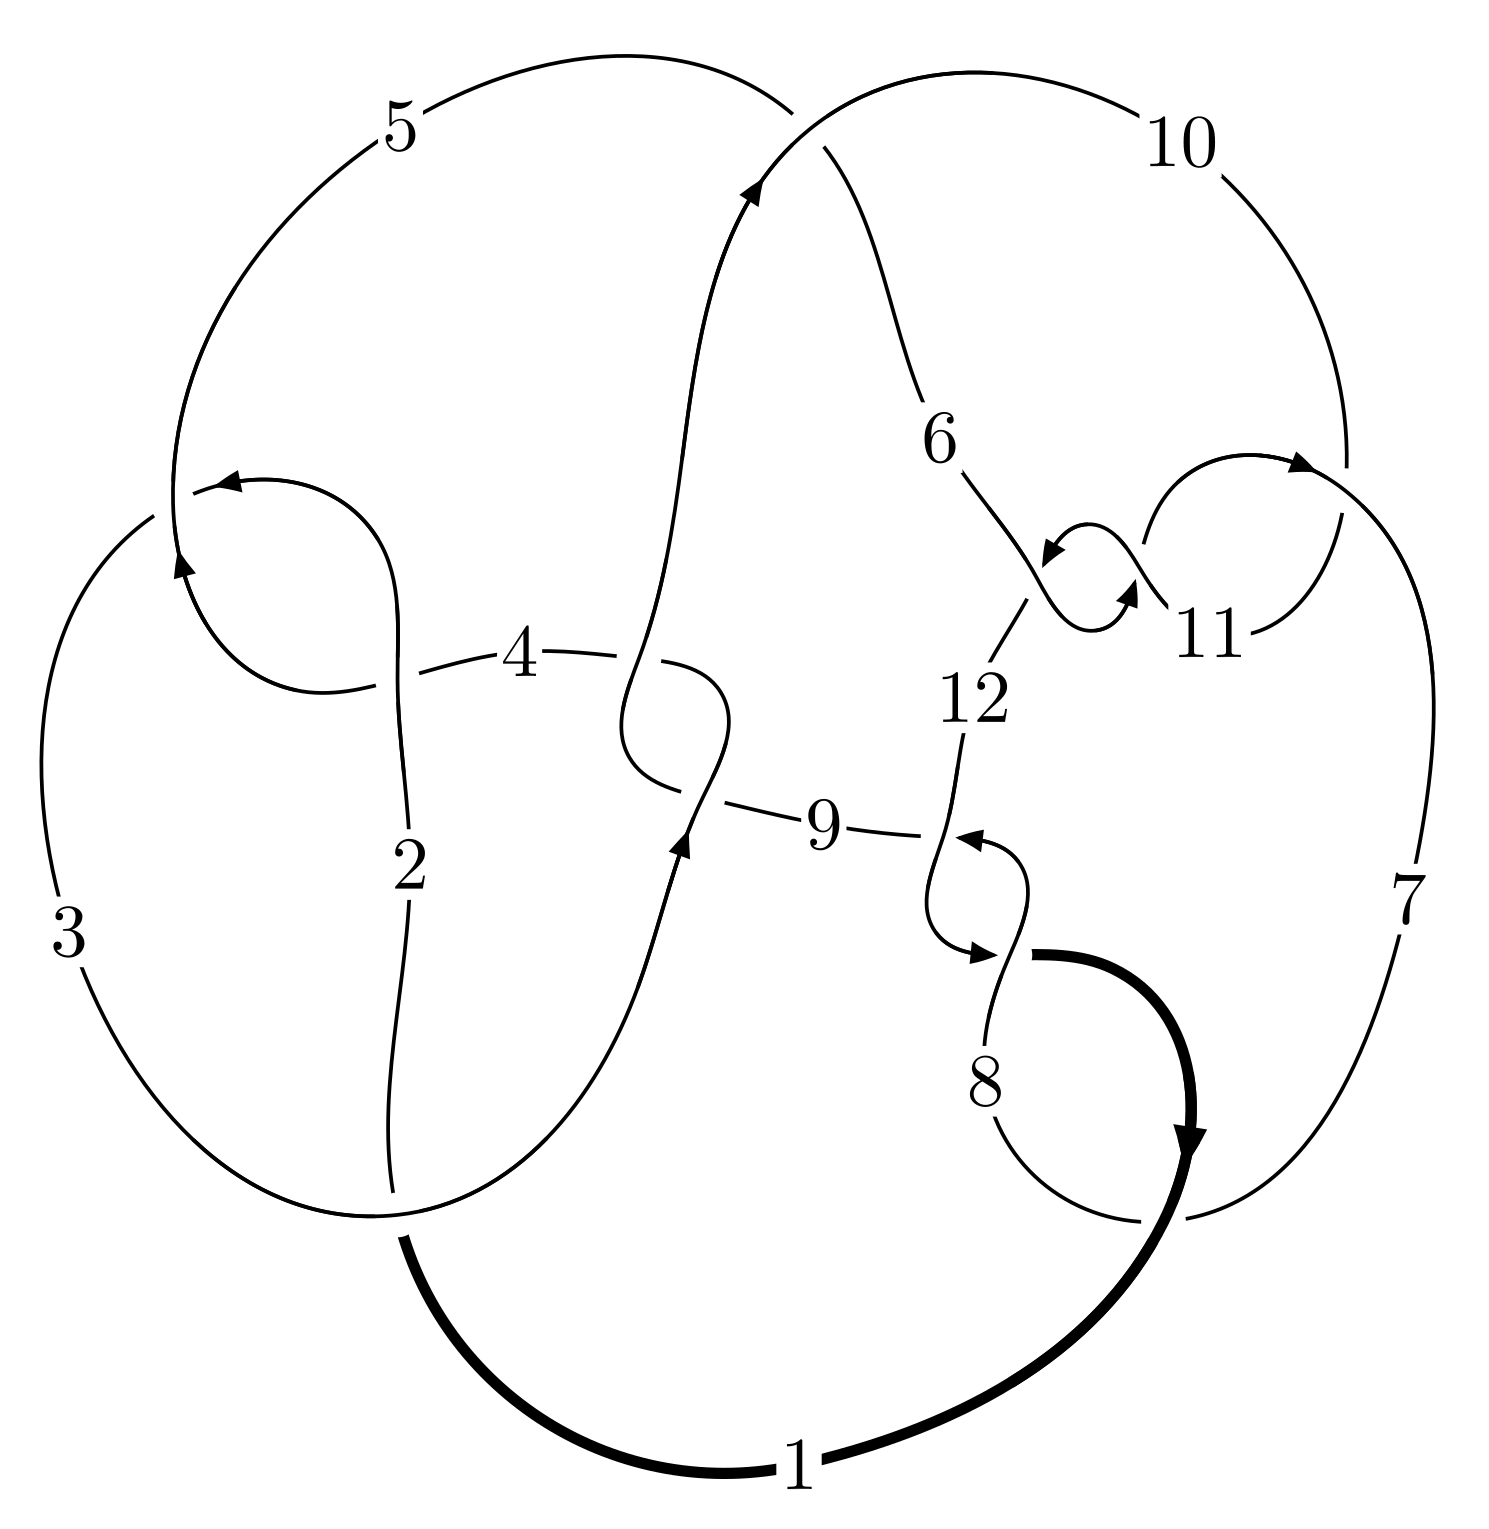
\includegraphics[width=112pt]{../../../GIT/diagram.site/Diagrams/png/2335_12n_0246.png}\\
\ \ \ A knot diagram\footnotemark}&
\allowdisplaybreaks
\textbf{Linearized knot diagam} \\
\cline{2-2}
 &
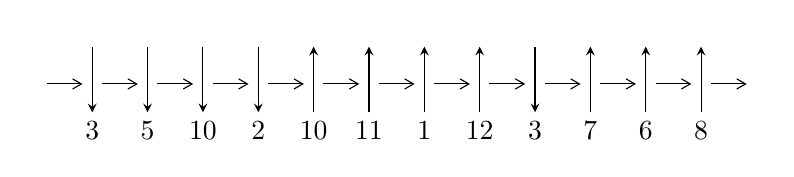
\begin{tikzpicture}[x=20pt, y=17pt]
	% nodes
	\node (C0) at (0, 0) {};
	\node (C1) at (1, 0) {};
	\node (C1U) at (1, +1) {};
	\node (C1D) at (1, -1) {3};

	\node (C2) at (2, 0) {};
	\node (C2U) at (2, +1) {};
	\node (C2D) at (2, -1) {5};

	\node (C3) at (3, 0) {};
	\node (C3U) at (3, +1) {};
	\node (C3D) at (3, -1) {10};

	\node (C4) at (4, 0) {};
	\node (C4U) at (4, +1) {};
	\node (C4D) at (4, -1) {2};

	\node (C5) at (5, 0) {};
	\node (C5U) at (5, +1) {};
	\node (C5D) at (5, -1) {10};

	\node (C6) at (6, 0) {};
	\node (C6U) at (6, +1) {};
	\node (C6D) at (6, -1) {11};

	\node (C7) at (7, 0) {};
	\node (C7U) at (7, +1) {};
	\node (C7D) at (7, -1) {1};

	\node (C8) at (8, 0) {};
	\node (C8U) at (8, +1) {};
	\node (C8D) at (8, -1) {12};

	\node (C9) at (9, 0) {};
	\node (C9U) at (9, +1) {};
	\node (C9D) at (9, -1) {3};

	\node (C10) at (10, 0) {};
	\node (C10U) at (10, +1) {};
	\node (C10D) at (10, -1) {7};

	\node (C11) at (11, 0) {};
	\node (C11U) at (11, +1) {};
	\node (C11D) at (11, -1) {6};

	\node (C12) at (12, 0) {};
	\node (C12U) at (12, +1) {};
	\node (C12D) at (12, -1) {8};
	\node (C13) at (13, 0) {};

	% arrows
	\draw[->,>={angle 60}]
	(C0) edge (C1) (C1) edge (C2) (C2) edge (C3) (C3) edge (C4) (C4) edge (C5) (C5) edge (C6) (C6) edge (C7) (C7) edge (C8) (C8) edge (C9) (C9) edge (C10) (C10) edge (C11) (C11) edge (C12) (C12) edge (C13) ;	\draw[->,>=stealth]
	(C1U) edge (C1D) (C2U) edge (C2D) (C3U) edge (C3D) (C4U) edge (C4D) (C5D) edge (C5U) (C6D) edge (C6U) (C7D) edge (C7U) (C8D) edge (C8U) (C9U) edge (C9D) (C10D) edge (C10U) (C11D) edge (C11U) (C12D) edge (C12U) ;
	\end{tikzpicture} \\
\hhline{~~} \\& 
\textbf{Solving Sequence} \\ \cline{2-2} 
 &
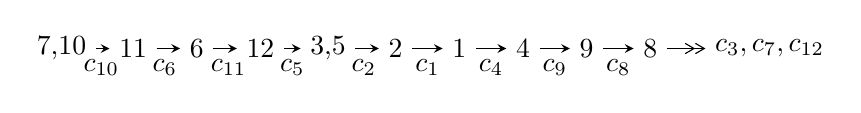
\begin{tikzpicture}[x=23pt, y=7pt]
	% node
	\node (A0) at (-1/8, 0) {7,10};
	\node (A1) at (1, 0) {11};
	\node (A2) at (2, 0) {6};
	\node (A3) at (3, 0) {12};
	\node (A4) at (65/16, 0) {3,5};
	\node (A5) at (41/8, 0) {2};
	\node (A6) at (49/8, 0) {1};
	\node (A7) at (57/8, 0) {4};
	\node (A8) at (65/8, 0) {9};
	\node (A9) at (73/8, 0) {8};
	\node (C1) at (1/2, -1) {$c_{10}$};
	\node (C2) at (3/2, -1) {$c_{6}$};
	\node (C3) at (5/2, -1) {$c_{11}$};
	\node (C4) at (7/2, -1) {$c_{5}$};
	\node (C5) at (37/8, -1) {$c_{2}$};
	\node (C6) at (45/8, -1) {$c_{1}$};
	\node (C7) at (53/8, -1) {$c_{4}$};
	\node (C8) at (61/8, -1) {$c_{9}$};
	\node (C9) at (69/8, -1) {$c_{8}$};
	\node (A10) at (11, 0) {$c_{3},c_{7},c_{12}$};

	% edge
	\draw[->,>=stealth]	
	(A0) edge (A1) (A1) edge (A2) (A2) edge (A3) (A3) edge (A4) (A4) edge (A5) (A5) edge (A6) (A6) edge (A7) (A7) edge (A8) (A8) edge (A9) ;
	\draw[->>,>={angle 60}]	
	(A9) edge (A10);
\end{tikzpicture} \\ 

\end{tabular} \\

\footnotetext{
The image of knot diagram is generated by the software ``\textbf{Draw programme}" developed by Andrew Bartholomew(\url{http://www.layer8.co.uk/maths/draw/index.htm\#Running-draw}), where we modified some parts for our purpose(\url{https://github.com/CATsTAILs/LinksPainter}).
}\phantom \\ \newline 
\centering \textbf{Ideals for irreducible components\footnotemark of $X_{\text{par}}$} 
 
\begin{align*}
I^u_{1}&=\langle 
u^{14}+u^{13}+6 u^{12}+6 u^{11}+15 u^{10}+14 u^9+19 u^8+13 u^7+9 u^6+3 u^5-5 u^4-2 u^3-5 u^2+2 b+1,\\
\phantom{I^u_{1}}&\phantom{= \langle  }u^{14}-3 u^{13}+\cdots+8 a+19,\\
\phantom{I^u_{1}}&\phantom{= \langle  }u^{15}+7 u^{13}+2 u^{12}+19 u^{11}+13 u^{10}+23 u^9+30 u^8+10 u^7+26 u^6- u^4+3 u^3-9 u^2+3 u+1\rangle \\
I^u_{2}&=\langle 
-716717 u^{25}+780792 u^{24}+\cdots+963947 b+791849,\\
\phantom{I^u_{2}}&\phantom{= \langle  }1775750 u^{25}-1897723 u^{24}+\cdots+963947 a-1845988,\;u^{26}-2 u^{25}+\cdots-2 u+1\rangle \\
I^u_{3}&=\langle 
b,\;- u^2+2 a- u-3,\;u^3+2 u-1\rangle \\
I^u_{4}&=\langle 
b,\;u^3+a+u+1,\;u^4+u^3+2 u^2+2 u+1\rangle \\
\\
\end{align*}
\raggedright * 4 irreducible components of $\dim_{\mathbb{C}}=0$, with total 48 representations.\\
\footnotetext{All coefficients of polynomials are rational numbers. But the coefficients are sometimes approximated in decimal forms when there is not enough margin.}
\newpage
\renewcommand{\arraystretch}{1}
\centering \section*{I. $I^u_{1}= \langle u^{14}+u^{13}+\cdots+2 b+1,\;u^{14}-3 u^{13}+\cdots+8 a+19,\;u^{15}+7 u^{13}+\cdots+3 u+1 \rangle$}
\flushleft \textbf{(i) Arc colorings}\\
\begin{tabular}{m{7pt} m{180pt} m{7pt} m{180pt} }
\flushright $a_{7}=$&$\begin{pmatrix}0\\u\end{pmatrix}$ \\
\flushright $a_{10}=$&$\begin{pmatrix}1\\0\end{pmatrix}$ \\
\flushright $a_{11}=$&$\begin{pmatrix}1\\- u^2\end{pmatrix}$ \\
\flushright $a_{6}=$&$\begin{pmatrix}- u\\u^3+u\end{pmatrix}$ \\
\flushright $a_{12}=$&$\begin{pmatrix}u^2+1\\- u^4-2 u^2\end{pmatrix}$ \\
\flushright $a_{3}=$&$\begin{pmatrix}-\frac{1}{8} u^{14}+\frac{3}{8} u^{13}+\cdots+5 u-\frac{19}{8}\\-\frac{1}{2} u^{14}-\frac{1}{2} u^{13}+\cdots+\frac{5}{2} u^2-\frac{1}{2}\end{pmatrix}$ \\
\flushright $a_{5}=$&$\begin{pmatrix}- u^3-2 u\\u^3+u\end{pmatrix}$ \\
\flushright $a_{2}=$&$\begin{pmatrix}-\frac{3}{8} u^{14}+\frac{1}{8} u^{13}+\cdots+4 u-\frac{25}{8}\\u^3+u\end{pmatrix}$ \\
\flushright $a_{1}=$&$\begin{pmatrix}-1\\u^{13}+6 u^{11}+2 u^{10}+13 u^9+11 u^8+10 u^7+19 u^6+7 u^4-7 u^2+3 u+1\end{pmatrix}$ \\
\flushright $a_{4}=$&$\begin{pmatrix}\frac{3}{8} u^{14}+\frac{7}{8} u^{13}+\cdots+5 u-\frac{15}{8}\\-\frac{1}{2} u^{14}-\frac{1}{2} u^{13}+\cdots+\frac{5}{2} u^2-\frac{1}{2}\end{pmatrix}$ \\
\flushright $a_{9}=$&$\begin{pmatrix}u^3+2 u\\- u^{14}-6 u^{12}-2 u^{11}-13 u^{10}-11 u^9-10 u^8-19 u^7-8 u^5+5 u^3-3 u^2\end{pmatrix}$ \\
\flushright $a_{8}=$&$\begin{pmatrix}u\\- u^{14}-6 u^{12}-2 u^{11}-13 u^{10}-11 u^9-10 u^8-19 u^7-7 u^5+7 u^3-3 u^2\end{pmatrix}$\\&\end{tabular}
\flushleft \textbf{(ii) Obstruction class $= -1$}\\~\\
\flushleft \textbf{(iii) Cusp Shapes $= -\frac{49}{16} u^{14}-\frac{45}{16} u^{13}-22 u^{12}-\frac{177}{8} u^{11}-\frac{1069}{16} u^{10}-\frac{579}{8} u^9-\frac{1701}{16} u^8-\frac{1839}{16} u^7-\frac{1341}{16} u^6-\frac{1299}{16} u^5-\frac{199}{16} u^4-\frac{29}{8} u^3+\frac{267}{16} u^2+\frac{37}{2} u-\frac{123}{16}$}\\~\\
\newpage\renewcommand{\arraystretch}{1}
\flushleft \textbf{(iv) u-Polynomials at the component}\newline \\
\begin{tabular}{m{50pt}|m{274pt}}
Crossings & \hspace{64pt}u-Polynomials at each crossing \\
\hline $$\begin{aligned}c_{1}\end{aligned}$$&$\begin{aligned}
&u^{15}+4 u^{14}+\cdots-127 u+16
\end{aligned}$\\
\hline $$\begin{aligned}c_{2},c_{4}\end{aligned}$$&$\begin{aligned}
&u^{15}-2 u^{14}+\cdots-11 u+4
\end{aligned}$\\
\hline $$\begin{aligned}c_{3},c_{9}\end{aligned}$$&$\begin{aligned}
&u^{15}-3 u^{14}+\cdots+8 u+32
\end{aligned}$\\
\hline $$\begin{aligned}c_{5}\end{aligned}$$&$\begin{aligned}
&u^{15}+6 u^{14}+\cdots+16 u+4
\end{aligned}$\\
\hline $$\begin{aligned}c_{6},c_{7},c_{8}\\c_{10},c_{11},c_{12}\end{aligned}$$&$\begin{aligned}
&u^{15}+7 u^{13}+\cdots+3 u+1
\end{aligned}$\\
\hline
\end{tabular}\\~\\
\newpage\renewcommand{\arraystretch}{1}
\flushleft \textbf{(v) Riley Polynomials at the component}\newline \\
\begin{tabular}{m{50pt}|m{274pt}}
Crossings & \hspace{64pt}Riley Polynomials at each crossing \\
\hline $$\begin{aligned}c_{1}\end{aligned}$$&$\begin{aligned}
&y^{15}+16 y^{14}+\cdots+15841 y-256
\end{aligned}$\\
\hline $$\begin{aligned}c_{2},c_{4}\end{aligned}$$&$\begin{aligned}
&y^{15}-4 y^{14}+\cdots-127 y-16
\end{aligned}$\\
\hline $$\begin{aligned}c_{3},c_{9}\end{aligned}$$&$\begin{aligned}
&y^{15}+15 y^{14}+\cdots+320 y-1024
\end{aligned}$\\
\hline $$\begin{aligned}c_{5}\end{aligned}$$&$\begin{aligned}
&y^{15}-16 y^{14}+\cdots+408 y-16
\end{aligned}$\\
\hline $$\begin{aligned}c_{6},c_{7},c_{8}\\c_{10},c_{11},c_{12}\end{aligned}$$&$\begin{aligned}
&y^{15}+14 y^{14}+\cdots+27 y-1
\end{aligned}$\\
\hline
\end{tabular}\\~\\
\newpage\flushleft \textbf{(vi) Complex Volumes and Cusp Shapes}
$$\begin{array}{c|c|c}  
\text{Solutions to }I^u_{1}& \I (\text{vol} + \sqrt{-1}CS) & \text{Cusp shape}\\
 \hline 
\begin{aligned}
u &= -0.939067 + 0.076154 I \\
a &= \phantom{-}0.11949 - 2.06723 I \\
b &= \phantom{-}0.27318 + 1.76916 I\end{aligned}
 & \phantom{-}9.05174 - 3.68246 I & \phantom{-}5.44943 + 2.70726 I \\ \hline\begin{aligned}
u &= -0.939067 - 0.076154 I \\
a &= \phantom{-}0.11949 + 2.06723 I \\
b &= \phantom{-}0.27318 - 1.76916 I\end{aligned}
 & \phantom{-}9.05174 + 3.68246 I & \phantom{-}5.44943 - 2.70726 I \\ \hline\begin{aligned}
u &= -0.231015 + 1.209380 I \\
a &= \phantom{-}0.202894 - 0.516586 I \\
b &= \phantom{-}1.71816 + 0.21702 I\end{aligned}
 & -5.39974 - 5.30636 I & -4.44673 + 7.07969 I \\ \hline\begin{aligned}
u &= -0.231015 - 1.209380 I \\
a &= \phantom{-}0.202894 + 0.516586 I \\
b &= \phantom{-}1.71816 - 0.21702 I\end{aligned}
 & -5.39974 + 5.30636 I & -4.44673 - 7.07969 I \\ \hline\begin{aligned}
u &= \phantom{-}0.072090 + 1.233060 I \\
a &= -0.067666 + 0.756607 I \\
b &= -0.93944 - 1.48122 I\end{aligned}
 & -8.55605 + 1.99221 I & -8.96301 - 2.93013 I \\ \hline\begin{aligned}
u &= \phantom{-}0.072090 - 1.233060 I \\
a &= -0.067666 - 0.756607 I \\
b &= -0.93944 + 1.48122 I\end{aligned}
 & -8.55605 - 1.99221 I & -8.96301 + 2.93013 I \\ \hline\begin{aligned}
u &= \phantom{-}0.446281 + 1.234210 I \\
a &= -0.890631 - 0.905985 I \\
b &= -0.39141 + 1.88678 I\end{aligned}
 & \phantom{-}1.89371 + 6.18917 I & -0.33163 - 4.59933 I \\ \hline\begin{aligned}
u &= \phantom{-}0.446281 - 1.234210 I \\
a &= -0.890631 + 0.905985 I \\
b &= -0.39141 - 1.88678 I\end{aligned}
 & \phantom{-}1.89371 - 6.18917 I & -0.33163 + 4.59933 I \\ \hline\begin{aligned}
u &= \phantom{-}0.45365 + 1.36129 I \\
a &= \phantom{-}1.09428 + 1.03938 I \\
b &= \phantom{-}0.73653 - 1.65036 I\end{aligned}
 & \phantom{-}0.04752 + 13.68620 I & -2.00699 - 7.52630 I \\ \hline\begin{aligned}
u &= \phantom{-}0.45365 - 1.36129 I \\
a &= \phantom{-}1.09428 - 1.03938 I \\
b &= \phantom{-}0.73653 + 1.65036 I\end{aligned}
 & \phantom{-}0.04752 - 13.68620 I & -2.00699 + 7.52630 I\\
 \hline 
 \end{array}$$\newpage$$\begin{array}{c|c|c}  
\text{Solutions to }I^u_{1}& \I (\text{vol} + \sqrt{-1}CS) & \text{Cusp shape}\\
 \hline 
\begin{aligned}
u &= \phantom{-}0.511100 + 0.177219 I \\
a &= -0.649618 - 0.329498 I \\
b &= \phantom{-}0.434596 + 0.530398 I\end{aligned}
 & \phantom{-}1.055330 + 0.384583 I & \phantom{-}8.52259 - 2.33147 I \\ \hline\begin{aligned}
u &= \phantom{-}0.511100 - 0.177219 I \\
a &= -0.649618 + 0.329498 I \\
b &= \phantom{-}0.434596 - 0.530398 I\end{aligned}
 & \phantom{-}1.055330 - 0.384583 I & \phantom{-}8.52259 + 2.33147 I \\ \hline\begin{aligned}
u &= -0.21189 + 1.50842 I \\
a &= -0.299323 - 0.077409 I \\
b &= -0.130865 - 0.674935 I\end{aligned}
 & -10.59470 - 5.64919 I & \phantom{-}0.00874 + 7.25798 I \\ \hline\begin{aligned}
u &= -0.21189 - 1.50842 I \\
a &= -0.299323 + 0.077409 I \\
b &= -0.130865 + 0.674935 I\end{aligned}
 & -10.59470 + 5.64919 I & \phantom{-}0.00874 - 7.25798 I \\ \hline\begin{aligned}
u &= -0.202297\phantom{ +0.000000I} \\
a &= -3.51885\phantom{ +0.000000I} \\
b &= -0.401516\phantom{ +0.000000I}\end{aligned}
 & -1.31450\phantom{ +0.000000I} & -10.7150\phantom{ +0.000000I}\\
 \hline 
 \end{array}$$\newpage\newpage\renewcommand{\arraystretch}{1}
\centering \section*{II. $I^u_{2}= \langle -7.17\times10^{5} u^{25}+7.81\times10^{5} u^{24}+\cdots+9.64\times10^{5} b+7.92\times10^{5},\;1.78\times10^{6} u^{25}-1.90\times10^{6} u^{24}+\cdots+9.64\times10^{5} a-1.85\times10^{6},\;u^{26}-2 u^{25}+\cdots-2 u+1 \rangle$}
\flushleft \textbf{(i) Arc colorings}\\
\begin{tabular}{m{7pt} m{180pt} m{7pt} m{180pt} }
\flushright $a_{7}=$&$\begin{pmatrix}0\\u\end{pmatrix}$ \\
\flushright $a_{10}=$&$\begin{pmatrix}1\\0\end{pmatrix}$ \\
\flushright $a_{11}=$&$\begin{pmatrix}1\\- u^2\end{pmatrix}$ \\
\flushright $a_{6}=$&$\begin{pmatrix}- u\\u^3+u\end{pmatrix}$ \\
\flushright $a_{12}=$&$\begin{pmatrix}u^2+1\\- u^4-2 u^2\end{pmatrix}$ \\
\flushright $a_{3}=$&$\begin{pmatrix}-1.84217 u^{25}+1.96870 u^{24}+\cdots-7.48746 u+1.91503\\0.743523 u^{25}-0.809995 u^{24}+\cdots+3.02101 u-0.821465\end{pmatrix}$ \\
\flushright $a_{5}=$&$\begin{pmatrix}- u^3-2 u\\u^3+u\end{pmatrix}$ \\
\flushright $a_{2}=$&$\begin{pmatrix}-0.800732 u^{25}+0.943263 u^{24}+\cdots-3.90828 u+0.652479\\u^3+u\end{pmatrix}$ \\
\flushright $a_{1}=$&$\begin{pmatrix}-0.679349 u^{25}+0.982915 u^{24}+\cdots+5.45700 u+1.72423\\0.456267 u^{25}-0.655675 u^{24}+\cdots+0.0722156 u-1.37578\end{pmatrix}$ \\
\flushright $a_{4}=$&$\begin{pmatrix}-2.58569 u^{25}+2.77870 u^{24}+\cdots-10.5085 u+2.73650\\0.743523 u^{25}-0.809995 u^{24}+\cdots+3.02101 u-0.821465\end{pmatrix}$ \\
\flushright $a_{9}=$&$\begin{pmatrix}1.25686 u^{25}-1.88879 u^{24}+\cdots+1.53675 u-2.45627\\-0.476873 u^{25}+0.609237 u^{24}+\cdots+0.104718 u+0.401848\end{pmatrix}$ \\
\flushright $a_{8}=$&$\begin{pmatrix}0.624218 u^{25}-1.70470 u^{24}+\cdots+1.36553 u-1.32065\\0.632641 u^{25}-0.184085 u^{24}+\cdots+2.17122 u-1.13562\end{pmatrix}$\\&\end{tabular}
\flushleft \textbf{(ii) Obstruction class $= -1$}\\~\\
\flushleft \textbf{(iii) Cusp Shapes $= \frac{1918707}{963947} u^{25}-\frac{2455152}{963947} u^{24}+\cdots-\frac{5103125}{963947} u+\frac{1698759}{963947}$}\\~\\
\newpage\renewcommand{\arraystretch}{1}
\flushleft \textbf{(iv) u-Polynomials at the component}\newline \\
\begin{tabular}{m{50pt}|m{274pt}}
Crossings & \hspace{64pt}u-Polynomials at each crossing \\
\hline $$\begin{aligned}c_{1}\end{aligned}$$&$\begin{aligned}
&(u^{13}+3 u^{12}+\cdots+8 u+1)^{2}
\end{aligned}$\\
\hline $$\begin{aligned}c_{2},c_{4}\end{aligned}$$&$\begin{aligned}
&(u^{13}-3 u^{12}+\cdots-2 u+1)^{2}
\end{aligned}$\\
\hline $$\begin{aligned}c_{3},c_{9}\end{aligned}$$&$\begin{aligned}
&(u^{13}+u^{12}+\cdots+4 u-4)^{2}
\end{aligned}$\\
\hline $$\begin{aligned}c_{5}\end{aligned}$$&$\begin{aligned}
&(u^{13}-2 u^{12}+\cdots+3 u-1)^{2}
\end{aligned}$\\
\hline $$\begin{aligned}c_{6},c_{7},c_{8}\\c_{10},c_{11},c_{12}\end{aligned}$$&$\begin{aligned}
&u^{26}-2 u^{25}+\cdots-2 u+1
\end{aligned}$\\
\hline
\end{tabular}\\~\\
\newpage\renewcommand{\arraystretch}{1}
\flushleft \textbf{(v) Riley Polynomials at the component}\newline \\
\begin{tabular}{m{50pt}|m{274pt}}
Crossings & \hspace{64pt}Riley Polynomials at each crossing \\
\hline $$\begin{aligned}c_{1}\end{aligned}$$&$\begin{aligned}
&(y^{13}+17 y^{12}+\cdots+8 y-1)^{2}
\end{aligned}$\\
\hline $$\begin{aligned}c_{2},c_{4}\end{aligned}$$&$\begin{aligned}
&(y^{13}-3 y^{12}+\cdots+8 y-1)^{2}
\end{aligned}$\\
\hline $$\begin{aligned}c_{3},c_{9}\end{aligned}$$&$\begin{aligned}
&(y^{13}+15 y^{12}+\cdots-56 y-16)^{2}
\end{aligned}$\\
\hline $$\begin{aligned}c_{5}\end{aligned}$$&$\begin{aligned}
&(y^{13}-16 y^{12}+\cdots+5 y-1)^{2}
\end{aligned}$\\
\hline $$\begin{aligned}c_{6},c_{7},c_{8}\\c_{10},c_{11},c_{12}\end{aligned}$$&$\begin{aligned}
&y^{26}+18 y^{25}+\cdots+30 y^2+1
\end{aligned}$\\
\hline
\end{tabular}\\~\\
\newpage\flushleft \textbf{(vi) Complex Volumes and Cusp Shapes}
$$\begin{array}{c|c|c}  
\text{Solutions to }I^u_{2}& \I (\text{vol} + \sqrt{-1}CS) & \text{Cusp shape}\\
 \hline 
\begin{aligned}
u &= \phantom{-}0.971054 + 0.087562 I \\
a &= \phantom{-}0.20122 - 1.96513 I \\
b &= -0.50699 + 1.66583 I\end{aligned}
 & \phantom{-}4.58598 + 8.60203 I & \phantom{-}1.58542 - 5.32797 I \\ \hline\begin{aligned}
u &= \phantom{-}0.971054 - 0.087562 I \\
a &= \phantom{-}0.20122 + 1.96513 I \\
b &= -0.50699 - 1.66583 I\end{aligned}
 & \phantom{-}4.58598 - 8.60203 I & \phantom{-}1.58542 + 5.32797 I \\ \hline\begin{aligned}
u &= -0.166889 + 1.040940 I \\
a &= \phantom{-}1.41794 - 1.71859 I \\
b &= \phantom{-}0.612460\phantom{ +0.000000I}\end{aligned}
 & -4.29290\phantom{ +0.000000I} & -6.11820 + 0. I\phantom{ +0.000000I} \\ \hline\begin{aligned}
u &= -0.166889 - 1.040940 I \\
a &= \phantom{-}1.41794 + 1.71859 I \\
b &= \phantom{-}0.612460\phantom{ +0.000000I}\end{aligned}
 & -4.29290\phantom{ +0.000000I} & -6.11820 + 0. I\phantom{ +0.000000I} \\ \hline\begin{aligned}
u &= \phantom{-}0.898765 + 0.068276 I \\
a &= -0.51103 - 2.01532 I \\
b &= \phantom{-}0.02169 + 1.76519 I\end{aligned}
 & \phantom{-}5.49041 - 1.38297 I & \phantom{-}2.93425 + 0.71622 I \\ \hline\begin{aligned}
u &= \phantom{-}0.898765 - 0.068276 I \\
a &= -0.51103 + 2.01532 I \\
b &= \phantom{-}0.02169 - 1.76519 I\end{aligned}
 & \phantom{-}5.49041 + 1.38297 I & \phantom{-}2.93425 - 0.71622 I \\ \hline\begin{aligned}
u &= -0.705153 + 0.526357 I \\
a &= \phantom{-}0.314624 - 0.599897 I \\
b &= -0.032142 + 0.650070 I\end{aligned}
 & -3.89003 - 2.36301 I & \phantom{-}2.56487 + 4.19898 I \\ \hline\begin{aligned}
u &= -0.705153 - 0.526357 I \\
a &= \phantom{-}0.314624 + 0.599897 I \\
b &= -0.032142 - 0.650070 I\end{aligned}
 & -3.89003 + 2.36301 I & \phantom{-}2.56487 - 4.19898 I \\ \hline\begin{aligned}
u &= -0.063428 + 1.135530 I \\
a &= \phantom{-}0.99806 + 1.21295 I \\
b &= \phantom{-}0.452299 - 0.637242 I\end{aligned}
 & -4.25522 - 0.99909 I & \phantom{-}0.456384 - 0.581912 I \\ \hline\begin{aligned}
u &= -0.063428 - 1.135530 I \\
a &= \phantom{-}0.99806 - 1.21295 I \\
b &= \phantom{-}0.452299 + 0.637242 I\end{aligned}
 & -4.25522 + 0.99909 I & \phantom{-}0.456384 + 0.581912 I\\
 \hline 
 \end{array}$$\newpage$$\begin{array}{c|c|c}  
\text{Solutions to }I^u_{2}& \I (\text{vol} + \sqrt{-1}CS) & \text{Cusp shape}\\
 \hline 
\begin{aligned}
u &= \phantom{-}0.239526 + 1.122350 I \\
a &= -0.582484 - 0.652382 I \\
b &= -0.997974 + 0.288600 I\end{aligned}
 & -1.68175 + 2.52293 I & \phantom{-}2.35428 - 4.38707 I \\ \hline\begin{aligned}
u &= \phantom{-}0.239526 - 1.122350 I \\
a &= -0.582484 + 0.652382 I \\
b &= -0.997974 - 0.288600 I\end{aligned}
 & -1.68175 - 2.52293 I & \phantom{-}2.35428 + 4.38707 I \\ \hline\begin{aligned}
u &= -0.485725 + 1.232220 I \\
a &= \phantom{-}0.968192 - 0.729255 I \\
b &= \phantom{-}0.02169 + 1.76519 I\end{aligned}
 & \phantom{-}5.49041 - 1.38297 I & \phantom{-}2.93425 + 0.71622 I \\ \hline\begin{aligned}
u &= -0.485725 - 1.232220 I \\
a &= \phantom{-}0.968192 + 0.729255 I \\
b &= \phantom{-}0.02169 - 1.76519 I\end{aligned}
 & \phantom{-}5.49041 + 1.38297 I & \phantom{-}2.93425 - 0.71622 I \\ \hline\begin{aligned}
u &= \phantom{-}0.527181 + 1.230800 I \\
a &= -0.968929 - 0.539477 I \\
b &= \phantom{-}0.25689 + 1.55234 I\end{aligned}
 & \phantom{-}1.07459 - 3.30324 I & -0.83610 + 2.39821 I \\ \hline\begin{aligned}
u &= \phantom{-}0.527181 - 1.230800 I \\
a &= -0.968929 + 0.539477 I \\
b &= \phantom{-}0.25689 - 1.55234 I\end{aligned}
 & \phantom{-}1.07459 + 3.30324 I & -0.83610 - 2.39821 I \\ \hline\begin{aligned}
u &= \phantom{-}0.101397 + 1.371440 I \\
a &= \phantom{-}0.241803 - 0.465532 I \\
b &= -0.032142 - 0.650070 I\end{aligned}
 & -3.89003 + 2.36301 I & \phantom{-}2.56487 - 4.19898 I \\ \hline\begin{aligned}
u &= \phantom{-}0.101397 - 1.371440 I \\
a &= \phantom{-}0.241803 + 0.465532 I \\
b &= -0.032142 + 0.650070 I\end{aligned}
 & -3.89003 - 2.36301 I & \phantom{-}2.56487 + 4.19898 I \\ \hline\begin{aligned}
u &= \phantom{-}0.408597 + 1.339370 I \\
a &= \phantom{-}1.32284 + 0.50744 I \\
b &= \phantom{-}0.25689 - 1.55234 I\end{aligned}
 & \phantom{-}1.07459 + 3.30324 I & -0.83610 - 2.39821 I \\ \hline\begin{aligned}
u &= \phantom{-}0.408597 - 1.339370 I \\
a &= \phantom{-}1.32284 - 0.50744 I \\
b &= \phantom{-}0.25689 + 1.55234 I\end{aligned}
 & \phantom{-}1.07459 - 3.30324 I & -0.83610 + 2.39821 I\\
 \hline 
 \end{array}$$\newpage$$\begin{array}{c|c|c}  
\text{Solutions to }I^u_{2}& \I (\text{vol} + \sqrt{-1}CS) & \text{Cusp shape}\\
 \hline 
\begin{aligned}
u &= -0.43667 + 1.34910 I \\
a &= -1.26249 + 0.83530 I \\
b &= -0.50699 - 1.66583 I\end{aligned}
 & \phantom{-}4.58598 - 8.60203 I & \phantom{-}1.58542 + 5.32797 I \\ \hline\begin{aligned}
u &= -0.43667 - 1.34910 I \\
a &= -1.26249 - 0.83530 I \\
b &= -0.50699 + 1.66583 I\end{aligned}
 & \phantom{-}4.58598 + 8.60203 I & \phantom{-}1.58542 - 5.32797 I \\ \hline\begin{aligned}
u &= -0.517741 + 0.054555 I \\
a &= \phantom{-}1.276610 - 0.533825 I \\
b &= -0.997974 - 0.288600 I\end{aligned}
 & -1.68175 - 2.52293 I & \phantom{-}2.35428 + 4.38707 I \\ \hline\begin{aligned}
u &= -0.517741 - 0.054555 I \\
a &= \phantom{-}1.276610 + 0.533825 I \\
b &= -0.997974 + 0.288600 I\end{aligned}
 & -1.68175 + 2.52293 I & \phantom{-}2.35428 - 4.38707 I \\ \hline\begin{aligned}
u &= \phantom{-}0.229089 + 0.294081 I \\
a &= \phantom{-}0.08363 - 4.21290 I \\
b &= \phantom{-}0.452299 + 0.637242 I\end{aligned}
 & -4.25522 + 0.99909 I & \phantom{-}0.456384 + 0.581912 I \\ \hline\begin{aligned}
u &= \phantom{-}0.229089 - 0.294081 I \\
a &= \phantom{-}0.08363 + 4.21290 I \\
b &= \phantom{-}0.452299 - 0.637242 I\end{aligned}
 & -4.25522 - 0.99909 I & \phantom{-}0.456384 - 0.581912 I\\
 \hline 
 \end{array}$$\newpage\newpage\renewcommand{\arraystretch}{1}
\centering \section*{III. $I^u_{3}= \langle b,\;- u^2+2 a- u-3,\;u^3+2 u-1 \rangle$}
\flushleft \textbf{(i) Arc colorings}\\
\begin{tabular}{m{7pt} m{180pt} m{7pt} m{180pt} }
\flushright $a_{7}=$&$\begin{pmatrix}0\\u\end{pmatrix}$ \\
\flushright $a_{10}=$&$\begin{pmatrix}1\\0\end{pmatrix}$ \\
\flushright $a_{11}=$&$\begin{pmatrix}1\\- u^2\end{pmatrix}$ \\
\flushright $a_{6}=$&$\begin{pmatrix}- u\\- u+1\end{pmatrix}$ \\
\flushright $a_{12}=$&$\begin{pmatrix}u^2+1\\- u\end{pmatrix}$ \\
\flushright $a_{3}=$&$\begin{pmatrix}\frac{1}{2} u^2+\frac{1}{2} u+\frac{3}{2}\\0\end{pmatrix}$ \\
\flushright $a_{5}=$&$\begin{pmatrix}-1\\- u+1\end{pmatrix}$ \\
\flushright $a_{2}=$&$\begin{pmatrix}\frac{1}{2} u^2+\frac{1}{2} u+\frac{5}{2}\\u-1\end{pmatrix}$ \\
\flushright $a_{1}=$&$\begin{pmatrix}1\\u-1\end{pmatrix}$ \\
\flushright $a_{4}=$&$\begin{pmatrix}\frac{1}{2} u^2+\frac{1}{2} u+\frac{3}{2}\\0\end{pmatrix}$ \\
\flushright $a_{9}=$&$\begin{pmatrix}1\\0\end{pmatrix}$ \\
\flushright $a_{8}=$&$\begin{pmatrix}u\\u^2\end{pmatrix}$\\&\end{tabular}
\flushleft \textbf{(ii) Obstruction class $= 1$}\\~\\
\flushleft \textbf{(iii) Cusp Shapes $= \frac{25}{4} u^2+\frac{11}{4} u+\frac{23}{4}$}\\~\\
\newpage\renewcommand{\arraystretch}{1}
\flushleft \textbf{(iv) u-Polynomials at the component}\newline \\
\begin{tabular}{m{50pt}|m{274pt}}
Crossings & \hspace{64pt}u-Polynomials at each crossing \\
\hline $$\begin{aligned}c_{1},c_{2}\end{aligned}$$&$\begin{aligned}
&(u-1)^3
\end{aligned}$\\
\hline $$\begin{aligned}c_{3},c_{9}\end{aligned}$$&$\begin{aligned}
&u^3
\end{aligned}$\\
\hline $$\begin{aligned}c_{4}\end{aligned}$$&$\begin{aligned}
&(u+1)^3
\end{aligned}$\\
\hline $$\begin{aligned}c_{5}\end{aligned}$$&$\begin{aligned}
&u^3+3 u^2+5 u+2
\end{aligned}$\\
\hline $$\begin{aligned}c_{6},c_{7},c_{8}\end{aligned}$$&$\begin{aligned}
&u^3+2 u+1
\end{aligned}$\\
\hline $$\begin{aligned}c_{10},c_{11},c_{12}\end{aligned}$$&$\begin{aligned}
&u^3+2 u-1
\end{aligned}$\\
\hline
\end{tabular}\\~\\
\newpage\renewcommand{\arraystretch}{1}
\flushleft \textbf{(v) Riley Polynomials at the component}\newline \\
\begin{tabular}{m{50pt}|m{274pt}}
Crossings & \hspace{64pt}Riley Polynomials at each crossing \\
\hline $$\begin{aligned}c_{1},c_{2},c_{4}\end{aligned}$$&$\begin{aligned}
&(y-1)^3
\end{aligned}$\\
\hline $$\begin{aligned}c_{3},c_{9}\end{aligned}$$&$\begin{aligned}
&y^3
\end{aligned}$\\
\hline $$\begin{aligned}c_{5}\end{aligned}$$&$\begin{aligned}
&y^3+y^2+13 y-4
\end{aligned}$\\
\hline $$\begin{aligned}c_{6},c_{7},c_{8}\\c_{10},c_{11},c_{12}\end{aligned}$$&$\begin{aligned}
&y^3+4 y^2+4 y-1
\end{aligned}$\\
\hline
\end{tabular}\\~\\
\newpage\flushleft \textbf{(vi) Complex Volumes and Cusp Shapes}
$$\begin{array}{c|c|c}  
\text{Solutions to }I^u_{3}& \I (\text{vol} + \sqrt{-1}CS) & \text{Cusp shape}\\
 \hline 
\begin{aligned}
u &= -0.22670 + 1.46771 I \\
a &= \phantom{-}0.335258 + 0.401127 I \\
b &= \phantom{-0.000000 } 0\end{aligned}
 & -11.08570 - 5.13794 I & -8.01583 - 0.12290 I \\ \hline\begin{aligned}
u &= -0.22670 - 1.46771 I \\
a &= \phantom{-}0.335258 - 0.401127 I \\
b &= \phantom{-0.000000 } 0\end{aligned}
 & -11.08570 + 5.13794 I & -8.01583 + 0.12290 I \\ \hline\begin{aligned}
u &= \phantom{-}0.453398\phantom{ +0.000000I} \\
a &= \phantom{-}1.82948\phantom{ +0.000000I} \\
b &= \phantom{-0.000000 } 0\end{aligned}
 & -0.857735\phantom{ +0.000000I} & \phantom{-}8.28170\phantom{ +0.000000I}\\
 \hline 
 \end{array}$$\newpage\newpage\renewcommand{\arraystretch}{1}
\centering \section*{IV. $I^u_{4}= \langle b,\;u^3+a+u+1,\;u^4+u^3+2 u^2+2 u+1 \rangle$}
\flushleft \textbf{(i) Arc colorings}\\
\begin{tabular}{m{7pt} m{180pt} m{7pt} m{180pt} }
\flushright $a_{7}=$&$\begin{pmatrix}0\\u\end{pmatrix}$ \\
\flushright $a_{10}=$&$\begin{pmatrix}1\\0\end{pmatrix}$ \\
\flushright $a_{11}=$&$\begin{pmatrix}1\\- u^2\end{pmatrix}$ \\
\flushright $a_{6}=$&$\begin{pmatrix}- u\\u^3+u\end{pmatrix}$ \\
\flushright $a_{12}=$&$\begin{pmatrix}u^2+1\\u^3+2 u+1\end{pmatrix}$ \\
\flushright $a_{3}=$&$\begin{pmatrix}- u^3- u-1\\0\end{pmatrix}$ \\
\flushright $a_{5}=$&$\begin{pmatrix}- u^3-2 u\\u^3+u\end{pmatrix}$ \\
\flushright $a_{2}=$&$\begin{pmatrix}u-1\\- u^3- u\end{pmatrix}$ \\
\flushright $a_{1}=$&$\begin{pmatrix}u^3+2 u\\- u^3- u\end{pmatrix}$ \\
\flushright $a_{4}=$&$\begin{pmatrix}- u^3- u-1\\0\end{pmatrix}$ \\
\flushright $a_{9}=$&$\begin{pmatrix}1\\0\end{pmatrix}$ \\
\flushright $a_{8}=$&$\begin{pmatrix}2 u^3+u^2+3 u+3\\- u^3- u^2- u-2\end{pmatrix}$\\&\end{tabular}
\flushleft \textbf{(ii) Obstruction class $= 1$}\\~\\
\flushleft \textbf{(iii) Cusp Shapes $= 4 u^3+4 u-3$}\\~\\
\newpage\renewcommand{\arraystretch}{1}
\flushleft \textbf{(iv) u-Polynomials at the component}\newline \\
\begin{tabular}{m{50pt}|m{274pt}}
Crossings & \hspace{64pt}u-Polynomials at each crossing \\
\hline $$\begin{aligned}c_{1},c_{2}\end{aligned}$$&$\begin{aligned}
&(u-1)^4
\end{aligned}$\\
\hline $$\begin{aligned}c_{3},c_{9}\end{aligned}$$&$\begin{aligned}
&u^4
\end{aligned}$\\
\hline $$\begin{aligned}c_{4}\end{aligned}$$&$\begin{aligned}
&(u+1)^4
\end{aligned}$\\
\hline $$\begin{aligned}c_{5}\end{aligned}$$&$\begin{aligned}
&(u^2- u+1)^2
\end{aligned}$\\
\hline $$\begin{aligned}c_{6},c_{7},c_{8}\end{aligned}$$&$\begin{aligned}
&u^4- u^3+2 u^2-2 u+1
\end{aligned}$\\
\hline $$\begin{aligned}c_{10},c_{11},c_{12}\end{aligned}$$&$\begin{aligned}
&u^4+u^3+2 u^2+2 u+1
\end{aligned}$\\
\hline
\end{tabular}\\~\\
\newpage\renewcommand{\arraystretch}{1}
\flushleft \textbf{(v) Riley Polynomials at the component}\newline \\
\begin{tabular}{m{50pt}|m{274pt}}
Crossings & \hspace{64pt}Riley Polynomials at each crossing \\
\hline $$\begin{aligned}c_{1},c_{2},c_{4}\end{aligned}$$&$\begin{aligned}
&(y-1)^4
\end{aligned}$\\
\hline $$\begin{aligned}c_{3},c_{9}\end{aligned}$$&$\begin{aligned}
&y^4
\end{aligned}$\\
\hline $$\begin{aligned}c_{5}\end{aligned}$$&$\begin{aligned}
&(y^2+y+1)^2
\end{aligned}$\\
\hline $$\begin{aligned}c_{6},c_{7},c_{8}\\c_{10},c_{11},c_{12}\end{aligned}$$&$\begin{aligned}
&y^4+3 y^3+2 y^2+1
\end{aligned}$\\
\hline
\end{tabular}\\~\\
\newpage\flushleft \textbf{(vi) Complex Volumes and Cusp Shapes}
$$\begin{array}{c|c|c}  
\text{Solutions to }I^u_{4}& \I (\text{vol} + \sqrt{-1}CS) & \text{Cusp shape}\\
 \hline 
\begin{aligned}
u &= -0.621744 + 0.440597 I \\
a &= -0.500000 - 0.866025 I \\
b &= \phantom{-0.000000 } 0\end{aligned}
 & -4.93480 - 2.02988 I & -5.00000 + 3.46410 I \\ \hline\begin{aligned}
u &= -0.621744 - 0.440597 I \\
a &= -0.500000 + 0.866025 I \\
b &= \phantom{-0.000000 } 0\end{aligned}
 & -4.93480 + 2.02988 I & -5.00000 - 3.46410 I \\ \hline\begin{aligned}
u &= \phantom{-}0.121744 + 1.306620 I \\
a &= -0.500000 + 0.866025 I \\
b &= \phantom{-0.000000 } 0\end{aligned}
 & -4.93480 + 2.02988 I & -5.00000 - 3.46410 I \\ \hline\begin{aligned}
u &= \phantom{-}0.121744 - 1.306620 I \\
a &= -0.500000 - 0.866025 I \\
b &= \phantom{-0.000000 } 0\end{aligned}
 & -4.93480 - 2.02988 I & -5.00000 + 3.46410 I\\
 \hline 
 \end{array}$$\newpage
\newpage\renewcommand{\arraystretch}{1}
\centering \section*{ V. u-Polynomials}
\begin{tabular}{m{50pt}|m{274pt}}
Crossings & \hspace{64pt}u-Polynomials at each crossing \\
\hline $$\begin{aligned}c_{1}\end{aligned}$$&$\begin{aligned}
&((u-1)^7)(u^{13}+3 u^{12}+\cdots+8 u+1)^{2}(u^{15}+4 u^{14}+\cdots-127 u+16)
\end{aligned}$\\
\hline $$\begin{aligned}c_{2}\end{aligned}$$&$\begin{aligned}
&((u-1)^7)(u^{13}-3 u^{12}+\cdots-2 u+1)^{2}(u^{15}-2 u^{14}+\cdots-11 u+4)
\end{aligned}$\\
\hline $$\begin{aligned}c_{3},c_{9}\end{aligned}$$&$\begin{aligned}
&u^7(u^{13}+u^{12}+\cdots+4 u-4)^{2}(u^{15}-3 u^{14}+\cdots+8 u+32)
\end{aligned}$\\
\hline $$\begin{aligned}c_{4}\end{aligned}$$&$\begin{aligned}
&((u+1)^7)(u^{13}-3 u^{12}+\cdots-2 u+1)^{2}(u^{15}-2 u^{14}+\cdots-11 u+4)
\end{aligned}$\\
\hline $$\begin{aligned}c_{5}\end{aligned}$$&$\begin{aligned}
&((u^2- u+1)^2)(u^3+3 u^2+5 u+2)(u^{13}-2 u^{12}+\cdots+3 u-1)^{2}\\
&\cdot(u^{15}+6 u^{14}+\cdots+16 u+4)
\end{aligned}$\\
\hline $$\begin{aligned}c_{6},c_{7},c_{8}\end{aligned}$$&$\begin{aligned}
&(u^3+2 u+1)(u^4- u^3+2 u^2-2 u+1)(u^{15}+7 u^{13}+\cdots+3 u+1)\\
&\cdot(u^{26}-2 u^{25}+\cdots-2 u+1)
\end{aligned}$\\
\hline $$\begin{aligned}c_{10},c_{11},c_{12}\end{aligned}$$&$\begin{aligned}
&(u^3+2 u-1)(u^4+u^3+2 u^2+2 u+1)(u^{15}+7 u^{13}+\cdots+3 u+1)\\
&\cdot(u^{26}-2 u^{25}+\cdots-2 u+1)
\end{aligned}$\\
\hline
\end{tabular}\newpage\renewcommand{\arraystretch}{1}
\centering \section*{ VI. Riley Polynomials}
\begin{tabular}{m{50pt}|m{274pt}}
Crossings & \hspace{64pt}Riley Polynomials at each crossing \\
\hline $$\begin{aligned}c_{1}\end{aligned}$$&$\begin{aligned}
&((y-1)^7)(y^{13}+17 y^{12}+\cdots+8 y-1)^{2}\\
&\cdot(y^{15}+16 y^{14}+\cdots+15841 y-256)
\end{aligned}$\\
\hline $$\begin{aligned}c_{2},c_{4}\end{aligned}$$&$\begin{aligned}
&((y-1)^7)(y^{13}-3 y^{12}+\cdots+8 y-1)^{2}(y^{15}-4 y^{14}+\cdots-127 y-16)
\end{aligned}$\\
\hline $$\begin{aligned}c_{3},c_{9}\end{aligned}$$&$\begin{aligned}
&y^7(y^{13}+15 y^{12}+\cdots-56 y-16)^{2}(y^{15}+15 y^{14}+\cdots+320 y-1024)
\end{aligned}$\\
\hline $$\begin{aligned}c_{5}\end{aligned}$$&$\begin{aligned}
&((y^2+y+1)^2)(y^3+y^2+13 y-4)(y^{13}-16 y^{12}+\cdots+5 y-1)^{2}\\
&\cdot(y^{15}-16 y^{14}+\cdots+408 y-16)
\end{aligned}$\\
\hline $$\begin{aligned}c_{6},c_{7},c_{8}\\c_{10},c_{11},c_{12}\end{aligned}$$&$\begin{aligned}
&(y^3+4 y^2+4 y-1)(y^4+3 y^3+2 y^2+1)(y^{15}+14 y^{14}+\cdots+27 y-1)\\
&\cdot(y^{26}+18 y^{25}+\cdots+30 y^2+1)
\end{aligned}$\\
\hline
\end{tabular}
\vskip 2pc
\end{document}